\documentclass[12pt]{article}
\usepackage{float}
\usepackage{amsmath}
\usepackage{graphicx}
\usepackage{caption}
\usepackage{subcaption}
\usepackage{hyperref}
\usepackage[latin1]{inputenc}
\usepackage{geometry}
\geometry{
  a4paper,
  total={170mm,257mm},
  left=20mm,
  top=20mm,
}

\title{Requirements and Design Document}
\author{A project by Devs101\\ \\
Client: Mark-Anthony Fouché\\ \\
Christopher Njaravani\\
Charles Claassen\\
Dail Nathan Jonker\\
}
\date{14/10/2018}

\begin{document}
\maketitle
\begin{figure}[H]
	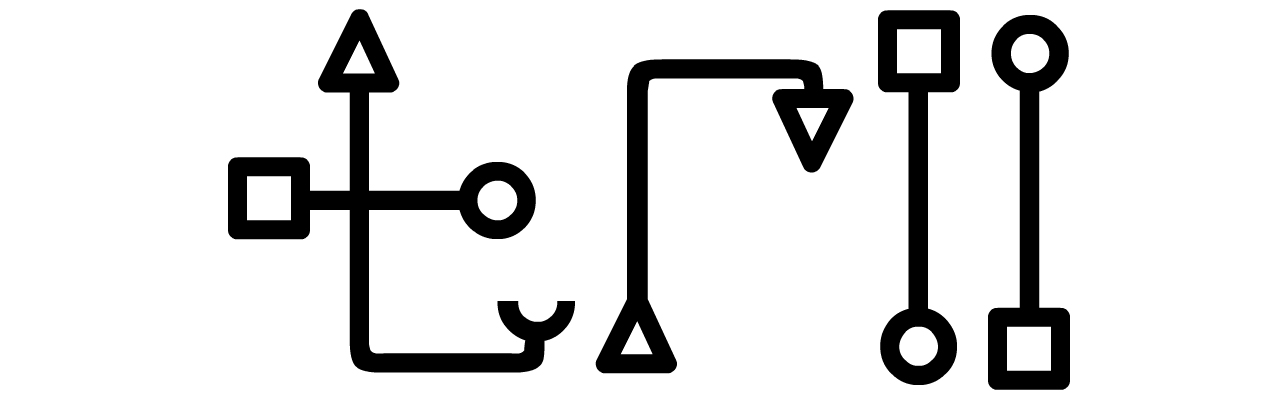
\includegraphics[width=\linewidth]{images/logo.jpg}
	\label{fig:logo}
\end{figure}
\newpage
\pagenumbering{arabic}

\tableofcontents
\newpage

\section{System Overview}

  \subsection{Purpose}
  The purpose of Trii is to provide users with a customizable skill tree creation platform for the use of gaming or live action role-playing. It allows users to create custom skills with custom rules, allowing them to build a skill tree the way they want.
  
  \subsection{Project scope}
  The scope of this project is to create a dynamic customizable skill tree. Nodes can be added, removed and information and rules regarding the node can be set and changed at any time.\newline 
  The layout of the tree can also be changed by dragging nodes around.\newline 
  Users can also add their own custom variables that can be used in calculations in the tree system.\newline 
  The tree also needs to store the state of the tree to support undo and redo functionality and also for offline work on the tree.
  \subsection{Definitions, acronyms and abbreviations}
  Gaming is video games or board games.\newline
  Live action role-playing is where people pretend to be part of a game or another world and sometimes dress up or just do things related to their game in the real world. This activity is usually called larping and the people that participate in it are called larpers.\newline
  Skill is a node in the tree and represents an ability your character can perform, example fireball skill, your character can cast fireballs.\newline
  Node is a point in a tree that can be interacted with and that represents a skill.\newline
  UI - User Interface, which is the components of the system the user will interact with.\newline
  API - Application programming interface.\newline
  MVC - Model-View-Controller. \newline
  \subsection{UML Domain model}
  
\begin{figure}[H]
  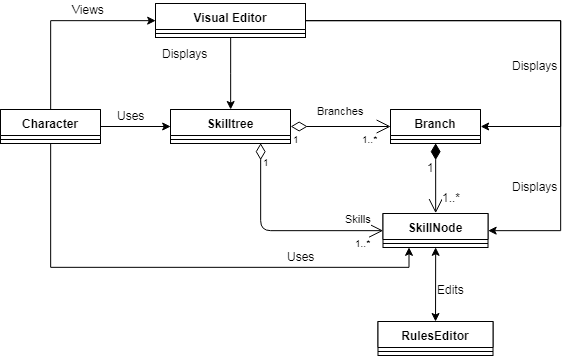
\includegraphics[width=\linewidth]{images/TriiDomainModel.png}
  \caption{The Domain model}
  \label{fig:Domainmodel}
\end{figure}
  
\section{Functional Requirements}
  \subsection{Users}
  Our users will be divided into four different user groups, namely:\newline\newline
  Game designers: These are the users that wish to create their own games and wish to user our system as their skill tree system in their games so that they do not have to make one from scratch. We assume these users have great computer skills and know how skill trees work and how to construct one and we also assume they have knowledge of programming and coding.\newline\newline
  Larpers: These are the users that participate in larping (Live action role playing). They can use the system to create and manage skill trees of their characters they created for their larping sessions. We assume that these users know the basics of a skill tree and how it works and how it should be structured.\newline\newline
  Gamers: These are users that play games (Video/board/card games or other type of games). These users can user this system to create and manage skill trees for their own gaming purposes. We assume that these users have basic computer knowledge and a good understanding of how skill trees work and how to use them.\newline\newline
  Others: These are the users that do not fall into any of our previous user groups. These users can use the system for any reason even if it is not game related like for example creating diagrams or family trees. We make no assumptions regarding these users, because we do not know anything about them.

  
  \subsection{Subsystems}
  The system is divided into five main subsystems with some subsystems of their own.\newline\newline
  Viewer:\newline
  This subsystem handles the display of the system (what the users will see). It will communicate with all the other subsystems to display their information in the proper format. The viewer will display the UI as well as the tree structure and update the view of the tree structure when it changes. Everything the user sees and interacts with is done through the viewer.\newline\newline
  Controller:\newline
  This subsystem manages the interaction of all the subsystems by sending and calculating information. The controller manages the UI and sends the information retrieved to the appropriate subsystem to handle the information. The controller also manages event handling and it is also responsible for updating the viewer on any changes made. The controller also initiates the Editor based on a UI instruction to edit a selected node's settings. The Controller is the heart of the system.
  \newline\newline
  Editor:\newline
  This subsystem manages the skill nodes. It handles creation, deletion and modification of the nodes. It communicates this information with the controller which then updates the viewer. The editor also stores the node data in the store and updates the Store when a nodes has been changed or deleted. It also allows functionality to select and modify multiple nodes at once. It also allows copies of nodes to be made.\newline\newline
  Simulator:\newline
  This subsystem is used for most of the systems calculations and data processing. The controller sends data and instructions to the Simulator and then it processes the data and executes the instructions. It gets any additional data needed from the store and once it is finished updates the store if any changes are made and sends a response to the controller, like a response to update the viewer. It also tests the data to make sure everything works as it should and if it finds an error it reports it to the controller to handle it. It is also responsible for creating the tree structure and all of its information and storing and updating that information in the store and it also communicates with the Editor through the Controller to editing some of the node settings and it tests the nodes and tree structure.\newline\newline
  Store:\newline
  This subsystem is the database of the system. This is where all the data is stored. The store does not do any data processing on its own, but it does provide the requested data for other subsystems. If the Controller is the heart then the Store is the blood that it pumps. The store is also divided into two subsystems which holds their own structures.\newline
  Tree data Structure:\newline 
  This subsystem of the store holds all the information relating to the tree. All the skills, their dependencies, the points spend in each skill and much more information is stored in this subsystem. This information is used by the viewer to display the tree.\newline
  Cytoscape Structure:\newline 
  This subsystem holds other important information regarding the framework we use as well as all the functions, variables, classes and other important information needed by the Simulator in order to run. This is the most important subsystem, because without it the system as a whole would not function.\newline \newline 
  Component UML Diagram:

  \begin{figure}[H]
    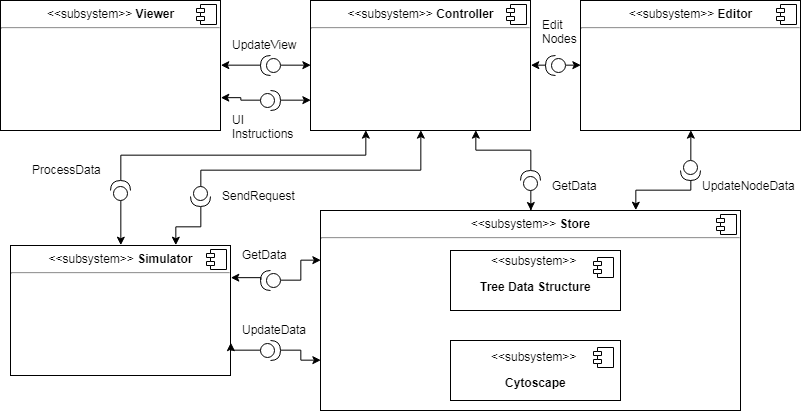
\includegraphics[width=\linewidth]{images/TriiUMLComponentDiagram}
    \caption{The UML Component Diagram}
    \label{fig:componentdiagram}
  \end{figure}


  \subsection{Specific requirements}
  \begin{enumerate}
  \item Viewer:
    \begin{enumerate}
      \item Display tree structure
      \item Provides the UI
      \item Retrieve data from UI and sends it to the controller
    \end{enumerate}
    \item Controller:
    \begin{enumerate}
      \item Retrieves and sends data to Viewer.
      \item Updates Viewer
      \item Sends data to the Store and updates Store
      \item Sends data to be processed by the Simulator
      \item Receives processed data from Simulator
      \item Handle errors retrieved from Simulator
      \item Facilitates interaction between components
      \item Initiates Editor on request
      \item Sends node related instructions to Editor
      \item Loads tree states with undo and redo requests
    \end{enumerate}
    \item Editor:
    \begin{enumerate}
      \item Add new nodes
      \item Delete existing nodes
      \item Move nodes
      \item Copy nodes
      \item Paste nodes
      \item Edit node settings:
      \begin{enumerate}
        \item Automatically generate an node ID
        \item Edit node name
        \item Edit node description
        \item Edit node visibility
        \item Edit node cost
        \item Edit node max skill point spend value
        \item Edit node dependencies
      \end{enumerate}
      \item Automatically creates links between nodes
      \item Stores all node data in Tree Data Structure Store
    \end{enumerate}
    \item Simulator:
    \begin{enumerate}
      \item Process data to be stored in Store
      \item Create global variables used in tree
      \item Test node settings and structure
      \item Test tree data structure
      \item Test global variables and test them on tree data structure
      \item Reports errors to controller
      \item Simulate tree data structure environment:
      \begin{enumerate}
        \item Create a tree data structure with appropriate settings and variables in place for the simulation
        \item Apply operations on simulated tree structure
        \item Report simulation success or failure
        \item Send simulation data to store and/or controller
      \end{enumerate}
    \end{enumerate}
    \item Store:
    \begin{enumerate}
      \item Stores all data
      \item Stores tree state objects
      \item Provides data to subsystem data request
      \item Manages and organizes stored data
      \item Allows queries on data.
      \item Allow stored data to be updated or removed
    \end{enumerate}
  \end{enumerate}

  Use Case Diagram:
  
  \begin{figure}[H]
    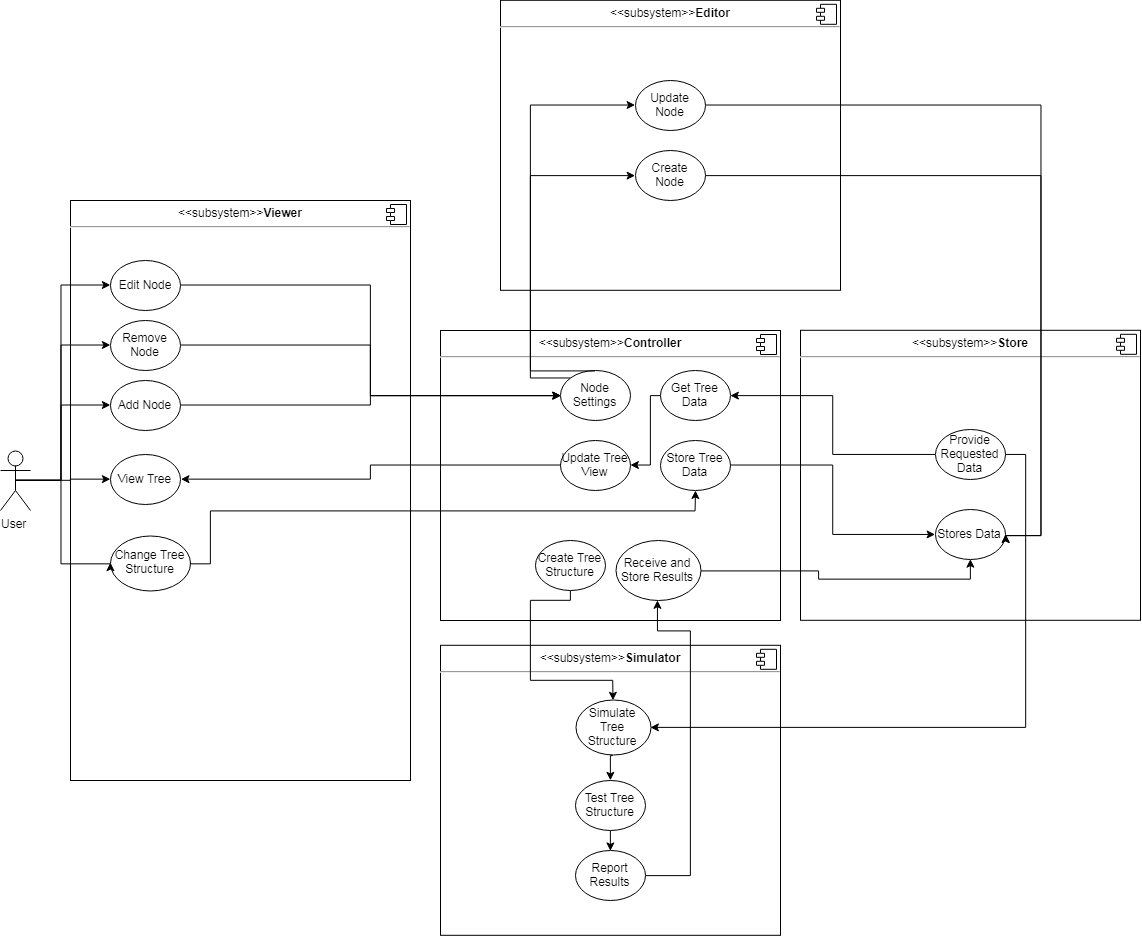
\includegraphics[width=\linewidth]{images/TriiUseCaseDiagram}
    \caption{Use Case Diagram}
    \label{fig:usecasediagram}
  \end{figure}

\section{Non-functional Requirements}
  The non-functional requirements we focus on is as follow:\newline\newline  
  Performance:\newline 
  This is focused on response and load time. How long it takes to load the page and the time it takes each operation to start and complete. We want the load/wait times to be as short as possible so users do not need to wait will using the system. This is important so that users will have a better experience using the system and not get bored or frustrated will using the system. This is achieved by optimizing our code and focusing on fast transfer of data as well as to make creating and updating the tree structure as fast as possible. The performance is tested when the tree is simulated and all the operations and actions performed during the simulation is timed to see how long it would take each action to occur and complete. If the results and total execution time is acceptable, no action takes more than 200 milliseconds, then the performance test is a success.\newline\newline  
  Availability:\newline 
  We want our system to be available at all times so anyone can use it at any time. We can achieve this by having the system hosted on a server that is always online and available for anyone to access and we even allow an offline version of our system to be downloaded on any device so this it can be used even if the user does not have a stable internet connection. We have tested the offline version that it works just as the online version and we check the server daily to make sure it is still online and that there are no problems with connections.\newline\newline  
  Usability:\newline 
  We want our system to be easy and simple to use. No need for a manual, although one is provided if needs be. We make sure we have a user friendly UI and that the flow of the website is straight forward. This is achieved by the use of simple layout and material design where we have simple, well labeled buttons for each core category that when clicked provide further buttons for more functionality. This saves screen space and compacts and groups the interaction better. All related functionality comes from one button making it easier for users to use. User can also interact with the tree itself and move just by clicking and dragging the node and one can edit and even delete individual nodes just by right clicking on the node to provide more options. This provides a very intuitive interaction with the tree and its nodes. Usability testing is done to get user feedback for improvements to the UI.\newline\newline  
  Cross Platform:\newline 
  Our system is based on a single page web application. Therefore it can be accessed using any browser on any operating system. We have tested the system on firefox and google chrome, however the framework we use should be compatible with any web browser, except internet explorer. We have also tested the systems on Windows, Linux, MacOS android and IOS. Some elements and icons may be displayed differently on the different operating systems, but they all work the same. The system is also optimized to work on mobile devices as well as desktop devices.\newline\newline  


\section{System Architecture}
  \subsection{Interfaces} 
    \subsubsection{User interfaces:} 
      The user interfaces of the system consist of:
      \begin{itemize}
      \item The tree viewer. The user will be able to directly interact with the tree to shape it into the form they want to have.
      \item The top bar menu. This provides the user with a fixed bar of buttons that provide the core and most simple functionality of the system. Buttons such as Undo, Redo, Copy, Paste and settings as well as a hamburger menu that provides additional options such as creating a new tree or importing an existing one and more.
      \item The floating buttons that provide more buttons like, add node, delete node, edit node etc. This allows for a more compact interface and provide each access to more functionality.
      \end{itemize}

    \subsubsection{Hardware interfaces:}
      Since our system is a web based system it does not interact with any hardware, it only interacts with the device's browser, so the browser manages the ports and sockets. The system uses an HTTPS protocol to connect with the device. The offline mode also uses the browser the run the system in a local host.

    \subsubsection{Software interfaces:}
      Our system uses the Vue framework and all of its required APIs. It is used for our system's structure and layout. We use the Cytoscape framework for creating, displaying and modifying our tree data structure. We use the Cypress framework and the Jest JavaScript library for testing our system. We also use Node.js and vuetify.js for creating our interface.

  \subsection{Architectural Styles} 
    The system as a whole uses the Client- Server architectural style, because the system is web based it is hosted on a server that clients can directly connect to and request the service from the server. The system also uses the MVC architectural pattern where the Viewer subsystem is the view that displays the information to the user such as the tree and all the nodes, as well as the UI. The Controller subsystem is of course the controller which take the input from the viewer and converts it to instructions for the model. It also manages the interaction between the subsystems. The model is the Store and the Editor subsystems. The Editor creates and modifies data and stores in in the Store where all the data is kept and organized. The Store subsystem also provides functionality for the data to be queried and requested.\newline\newline 
    Architectural styles applied for each subsystem is as follows:\newline\newline 
    Viewer: It makes use of only the MVC architectural pattern as described above.\newline\newline 
    Controller: It also only makes use of the MVC architectural pattern as described above.\newline \newline 
    Store: It makes use of the MVC architectural pattern as described above and also the Persistence framework architectural style for storing objects to a database and retrieving the objects per request of another subsystem. It has two different databases, which each function as their own sub system. There is a main database manager for the store and each database subsystem have their own database manager. The main database manager handles all incoming instructions and requests and then assigns them to the  database manager of the appropriate subsystem database.\newline \newline 
    Editor: It uses an Service-oriented architecture where the Editor provides a service to the Controller. The Controller receives instruction to create, delete or modify a node, then the Controller requests the services to perform this instruction from the Editor. In other words the Controller delegates all node related instructions to the Editor to perform.\newline \newline 
    Simulator: It also uses the Service-oriented architecture where it provides a service to the Controller. The service being to simulate and test the tree structure to make sure everything works as it should. The Simulator also makes use of the Event-driven architecture for the simulation of the tree. It takes the current state of the tree and simulates what would happen if certain events takes place, such as nodes changing, global variables (That define how the tree should funcion) are added or changed and the state of the tree resets and many more. Each event that takes place tests the tree to see if it responds appropriately or not and reports the results to the Controller.

  \subsection{System Configuration} 
    The system run on a Github server. It can be accessed through and computer or mobile device that can use a web browser. The web browser communicates with the website through a HTTPS protocol connection. The offline version of the system is downloaded onto the computer or mobile device and is then run using a browser in local host, so no internet connection is needed. The online system can update the offline system if the users allow the offline system to update, this will need an internet connection.\newline \newline 
    Deployment Diagram:
    
    \begin{figure}[H]
      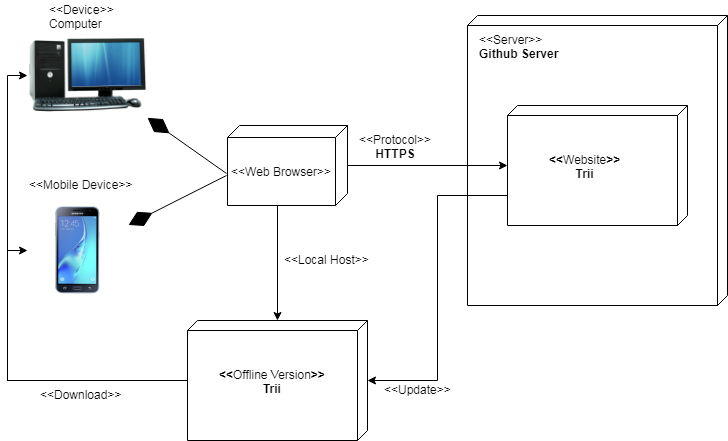
\includegraphics[width=\linewidth]{images/TriiDeploymentDiagram}
      \caption{The Deployment Diagram}
      \label{fig:deploymentdiagram}
    \end{figure}

\end{document}
